\chapter{Przedstawienie powiązanych algorytmów}
\label{cha:analizaTeoretycznaProblemu}
Algorytm, którego implementacja jest celem tejże pracy inżynierskiej można podzielić na kilka istotniejszych etapów. Kluczową kwestią jest moment wykrycia twarzy na obrazie, identyfikacja punktów charakterystycznych oraz zastosowanie triangulacji. Właśnie ze względu na  powyższe fakty, w kolejnych podrozdziałach opisane zostaną wymienione algorytmy, ich działanie oraz zastosowania. 

% %---------------------------------------------------------------------------

\section{Wykrywanie twarzy}
Poprzez pojęcie wykrywania twarzy (ang. face detection) \cite{fDetection} rozumie się opartą na sztucznej inteligencji technologię identyfikującą ludzkie twarze na obrazie cyfrowym. Nawiązując do wspomnianych wyżej faktów, owa technika używana jest w wielu rozbieżnych dziedzinach. Nie zawsze posługujemy się nią świadomie, w celu łatwego dostępu do różnego rodzaju sprzętu elektronicznego. Przedstawiana technologia otacza nas wszędzie.

Często wykorzystuje się ją w monitoringu wideo, aby zapewnić bezpieczeństwo osobiste jak i narodowe. Co za tym idzie, odpowiednie służby polegają na niej w momencie egzekwowania prawa lub identyfikacji osób w grupie. W dziedzinie marketingu zaczęto korzystać z personalizacji reklam dla danego użytkownika. Poprzez integrację kamery internetowej z telewizorem, można gromadzić informacje o osobie, lokalizując ją za pomocą detekcji twarzy. Zbiera się dane dotyczące rasy, płci oraz przedziału wiekowego, aby następnie na tej podstawie dostosować wyświetlane reklamy. W nowo powstających aparatach fotograficznych wykrywania twarzy używa się podczas automatycznego ustawiania ostrości. Nowoczesne urządzenia przez namierzenie uśmiechu, dobierają odpowiedni moment zrobienia zdjęcia, przez co odbywa się to bez manualnego użycia przycisków \cite{fDetection2}.

Na przestrzeni lat metody służące wykrywaniu twarzy bardzo się rozwinęły. Na początku używano podstawowych technik przetwarzania obrazów, następnie oparto je na uczeniu maszynowym. Aktualnie ważną rolę w efektywności tejże techniki odgrywają sieci neuronowe, których zastosowanie zdecydowanie przyspiesza działanie programów implementujących ową metodę.

Istnieje wiele różnych propozycji algorytmów służących wykrywaniu twarzy. W celu uporządkowania i pogrupowania metod stosuje się klasyfikację zawierającą cztery podstawowe techniki wykrywania twarzy na obrazie. Dany podział został zaproponowany w 2002 roku przez Ming-Hsuan Yanga (Rys. \ref{fig:detectionMethods}) i obowiązuje do dziś.

\begin{figure}[h]
	\centering
	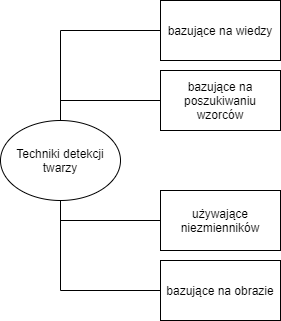
\includegraphics[width=7cm]{zdjęcia/techniki-detekcji.png}
	\caption{Techniki detekcji twarzy według Younga} 
	\label{fig:detectionMethods}
\end{figure}

Charakteryzację każdej z grup \cite{Yang} można przedstawić w następujący sposób:
\begin{itemize}
    \item metody bazujące na wiedzy - wykorzustujące ludzkie obeznanie na temat elementów jakie zawiera przeciętna twarz
    \item techniki używające niezmienników - algorytmy skupiają się na zlokalizowaniu cech strukturalnych twarzy, które są niezmienne ze względu na kąt, oświetlenie, pozycję twarzy
    \item metody bazujące na poszukiwaniu wzorców - dzięki wielu zgromadzonym wzorcom odnośnie wyglądu twarzy lub jej konkretnych elementów poszukuje się korelacji między schematem a obrazem wejściowym
    \item metody bazujące na obrazie - model trenowany jest zestawem obrazów, które zawierają różnorodne ludzkie twarze, przedstawiane w zmiennych warunkach
\end{itemize}

Zagadnienie poruszane w tym rozdziale jest bardzo rozległe, a rozwiązania i algorytmy istniejące na rynku bardzo różnorodne. Większość powstałych implementacji łączy najlepsze cechy z kilku metod, przez co nie ma możliwości przypisania ich do konkretnej klasyfikacji. Ze~względu na szeroki zakres tej 
tematyki oraz dużą ilość istniejących rozwiązań w dalszej części zostaną opisane dwa najpopularniejsze algorytmy, których implementacje są udostępniane przez biblioteki programistyczne.

% %---------------------------------------------------------------------------

\subsection{Schemat działania}
Dla omawianych poniżej algorytmów proces wykrywania twarzy odbywa się dwuetapowo. Początkowym etapem jest wyszkolenie klasyfikatora, którego zadaniem będzie wykrycie twarzy. 

Następnym jest uruchomienie detektora skanującego cały obraz w celu lokalizacji istotnych cech takich jak oczy, usta, nos czy brwi. Ich rozpoznanie możliwe jest przez zgromadzone informacje znajdujące się w wytrenowanym wcześniej modelu.

Większość algorytmów uzależnia swoją efektywność od wielkości danych, na których został przeszkolony klasyfikator. Trenowanie na dużych zbiorach danych poprawia zdolność algorytmu w trakcie określenia czy na danym obrazie znajduje się twarz \cite{fDetection}.

% %---------------------------------------------------------------------------

\subsection{Klasyfikator kaskadowy z użyciem cech Haara}
\label{sub:Haar}
Paul Viola i Michael Jones w 2001 roku zaproponowali technikę wykrywania obiektów opartą na działaniu klasyfikatora kaskad Haara (ang. Haar Feature-based Cascade Classifier)~\cite{haar}. Pomimo wysokiej konkurencji ze strony sieci neuronowych, algorytm cieszy się ogromną popularnością po dzień dzisiejszy. Jego zastosowanie okazało się być przełomem w dziedzinie wykrywania twarzy. 

Działanie tej techniki łączy ze sobą poniższe koncepcje:
\begin{itemize}
    \item poszukiwanie i wybór najdokładniejszych cech Haara,
    \item utworzenie zintegrowanych obrazów w celu szybkiego znalezienia danej cechy,
    \item użycie metody klasyfikacji Adaboost,
    \item zastosowanie klasyfikatora kaskadowego.
\end{itemize}

Podejście to jest oparte o wytrenowanie klasyfikatora kaskadowego na wielu pozytywnych i~negatywnych obrazach w skali szarości. Przez pierwszy rodzaj rozumie się zdjęcia zawierające twarze, natomiast jako próbki negatywne określa się zdjęcia, na których nie znajduje się twarz ludzka. Według zaleceń autorów algorytmu obrazy powinny mieć wymiary $24x24$ pikseli.

Pierwszym krokiem działania opisywanego modelu jest wydobycie ze wszystkich próbek odpowiednich cech Haara. Cechy te dotyczą zmian wartości kontrastu pomiędzy prostokątnymi grupami pikseli. W tym celu wykorzystuje się tak zwane funkcje Haara.

\begin{figure}[h]
	\centering
	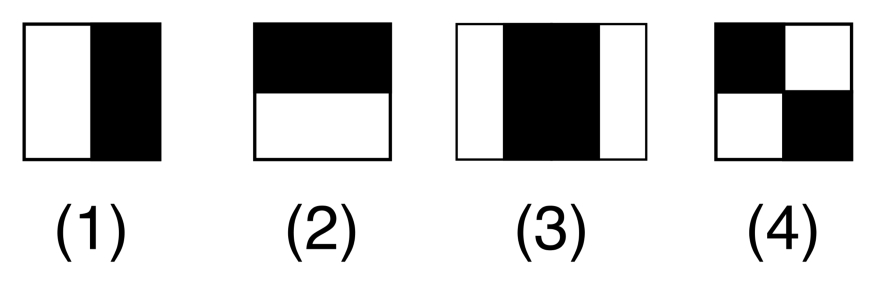
\includegraphics[width=6cm]{zdjęcia/haar_features.png}
	\caption{Przykładowe funkcje Haara \cite{haarCascade}} 
	\label{fig:haarFeatures}
\end{figure}

Są to kombinacje prostokątów  o takich samych wymiarach (ciemnych i jasnych), pozwalające na detekcję konkretnych elementów. Funkcje dzielimy na trzy grupy, ze względu na ilość prostokątów (2, 3, 4) tworzących daną cechę. Na Rys. \ref{fig:haarFeatures} przedstawiono funkcje używane w~tym algorytmie, wykorzystywane do wykrywania krawędzii na obrazie (1, 2) oraz prostych (3) i skośnych linii (4).

Każda funkcja Haara przemierza piksel po pikselu dany obraz. Dla każdego regionu (ciemnego jak i jasnego), który obejmuje owa cecha, sumowana jest wartość pikseli znajdujących się w tych obszarach. Następnie obliczana zostaje różnica między tymi sumami. Na podstawie tej różnicy, wyszukuje się lokalizację na obrazie, dla której dana cecha jest najbardziej odpowiednia. 

Przykładowo, na Rys. \ref{fig:haarNose} użyto funkcji złożonej z trzech prostokątów, o rozmiarze mającym na celu wykrycie oczu. Możliwe jest to poprzez fakt, iż obszar oczu jest ciemniejszy niż obszar nosa znajdujacy się pomiędzy nimi. Cechy Haara są pewnego rodzaju wzorcem, dla którego należy znaleźć najlepsze dopasowanie na obrazie.
 
\begin{figure}[h]
	\centering
	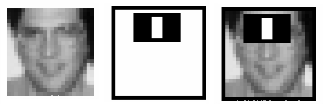
\includegraphics[width=5cm]{zdjęcia/haar_nose_feature.png}
	\caption{Zastosowanie funkcji Haara do wykrycia oczu i obszaru nosa \cite{haar}} 
	\label{fig:haarNose}
\end{figure}

Próba dopasowania cech Haara dla każdego piksela zawartego na obrazie, we wszystkich możliwych rozmiarach, wymaga wykonania niewyobrażalnej liczby działań. Rozwiązaniem jest stworzenie zintegrowanego obrazu, dzięki czemu złożoność obliczeń staje się dużo korzystniejsza.

Obrazem integralnym nazywamy reprezentację obrazu, w którym dana wartość $(x, y)$ równa jest sumie pikseli znajdujących się powyżej i na lewo od analizowanej lokalizacji (Rys. \ref{fig:integralImage}). Dana reprezentacja pozwala na przyspieszenie działań, jest to skuteczny sposób obliczenia sumy wartości pikseli dla prostokątnego podzbioru rozważanego obrazu.
 
 \begin{figure}[h]
	\centering
	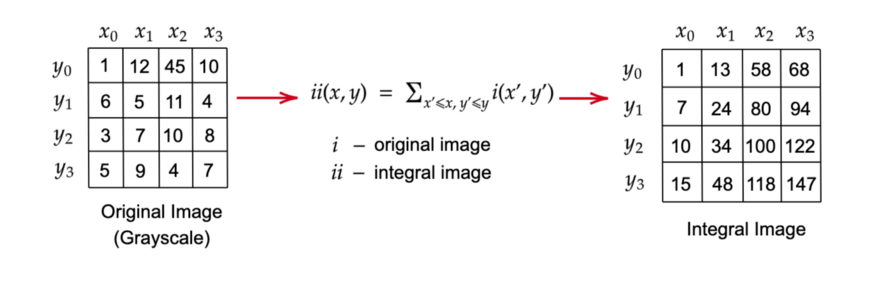
\includegraphics[width=14cm]{zdjęcia/integral.png}
	\caption{Konwersja na obraz zintegrowany \cite{haarCascade}} 
	\label{fig:integralImage}
\end{figure}
 
Kolejnym krokiem jest wybór cech, które są istotne dla konkretnych obszarów. Ten efekt można osiągnąć z pomocą algorytmu Adaboost (ang. Adaptive Boosting). Jest to  algorytm uczenia maszynowego służący do wyboru najlepszych funkcji z całego ich zbioru. Owa technika wzmacniająca, poprzez zastosowanie wszystkich możliwych cech na każdym obrazie treningowym osobno, wybiera te o najniższym błędzie dla danej iteracji. Algorytm trenuje silny klasyfikator na podstawie liniowej kombinacji słabych klasyfikatorów.
 
Po wyborze najlepszych cech spośród wszystkich możliwości pozostaje etap zastosowania klasyfikatora kaskadowego. Z definicji, działa on wielostopniowo. Cechy wybrane jako kluczowe zostają podzielone na grupy, gdzie każda z nich odpowiada jednemu etapowi działania klasyfikatora. Pierwsze etapy zawierają niewiele funkcji, ale wybrane zostają te najbardziej pewne i charakterystyczne. 
 
Funkcje są nakładane na każde okno o zadanych wymiarach wyodrębniane na obrazie. W~przypadku negatywnego rezultatu, tzn. niedopasowania jednej z cech sprawdzanych w konkretnym etapie, analizowane okno jest od razu odrzucane. Nie rozważa się dla niego funkcji zawartych w dalszych etapach. Jeśli natomiast okno przejdzie pomyślnie wszystkie etapy działania klasyfikatora kaskadowego zostaje zaklasyfikowane jako obszar twarzy (Rys. \ref{fig:cascadeClasificator}).  
 
\begin{figure}[h]
	\centering
	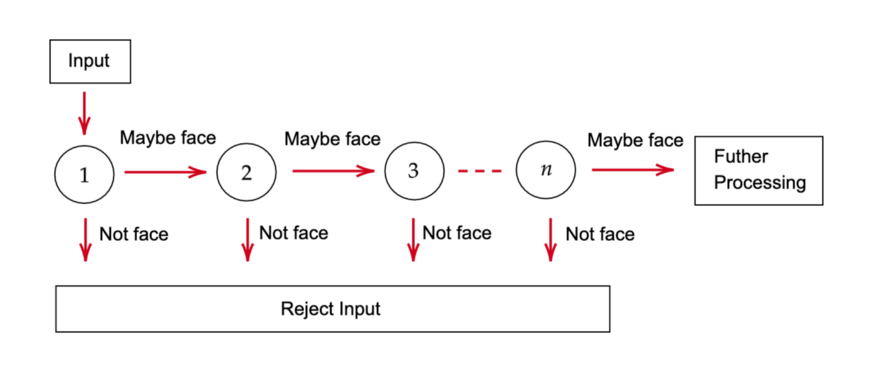
\includegraphics[width=14cm]{zdjęcia/haar_train.png}
	\caption{Klasyfikator kaskadowy \cite{haarCascade}} 
	\label{fig:cascadeClasificator}
\end{figure}

W badaniu przeprowadzonym przez autorów algorytmu wybrano 6000 funkcji, które podzielono na 38 etapów klasyfikacji. Liczba cech w każdym z nich nie jest proporcjonalna, wynosi ona kolejno 1, 10, 25, 25, 50 funkcji dla pięciu pierwszych etapów. W początkowych etapach eliminujemy okna, w których nie ma elementówch charakterystycznych twarzy. Oszczędza to zbędnych obliczeń i analiz.

Opisany w tym rozdziale algorytm jest wykorzystywany nie tylko do wykrywania twarzy na obrazach, ale także innego rodzaju obiektów, takich jak zwierzęta, tablice rejestracyjne czy całe ludzkie sylwetki. Cechuje go bardzo szybki czas działania. Jego dokładność nie jest aż tak wysoka, ze względu na podatność na fałszywe wykrycia.  Popularność algorytmu, który został opisany w tym rozdziale, zdaje się dalej trwać, pomimo odkrycia wielu konkurencyjnych rozwiązań działających na podobnej zasadzie. 

% %---------------------------------------------------------------------------

\subsection{Klasyfikator SVM z użyciem deskryptora HOG}
\label{sec:svmhog}
W 2005 roku pojawiła się kolejna przełomowa propozycja metody wykrywania obiektów, w tym twarzy. Jej autorami są Navneet Dalal i Bill Triggs, którzy wykazali, że do trenowania modelu można skorzystać z deskryptora HOG (ang. Histograms of Oriented Gradients) oraz klasyfikatora SVM (ang. Support Vector Machine) \cite{hog}. 

Deskryptory wyodrębniają z obrazu przydatne informacje pomijając zbędne dane, pomagają zlokalizować konkretny, interesujący nas obiekt. W przypadku deskryptorów HOG  ekstrakcja cech odbywa się za pomocą histogramu gradientów, używanych jako cechy analizowanych obrazów. Jako gradienty określamy pola wektorowe wskazujące kierunek, w którym można obserwować znaczącą zmianę w intensywności koloru.

W celu stworzenia deskryptora HOG dla obrazu należy wykonać kilka istotnych kroków \cite{hog2}. Pierwszym z nich jest przygotowanie obrazu w odcieniach szarości, dla którego chcemy obliczyć histogram gradientów. Według autorów algorytmu rozmiar zdjęcia powinno się zmniejszyć do $128x64$ pikseli. Takie wymiary zostały wybrane ze względu na początkowe przeznaczenie algorytmu. Miał on służyć do detekcji pieszych. Po sukcesie i otrzymaniu dobrych wyników, skupiono się na detekcji twarzy, w tym przypadku również zdecydowano się na wybór zdjęć o~owych wymiarach.

Dla każdego piksela znajdującego się na obrazie należy obliczyć gradient pionowy i poziomy. Najprostszym sposobem jest filtracja obrazu przez poniższe jądra.

\begin{figure}[h]
	\centering
	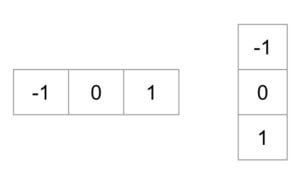
\includegraphics[width=5cm]{zdjęcia/hog-kernels.jpg}
	\caption{Jądra służące do filtracji obrazu w celu obliczenia gradientów \cite{hog2}} 
	\label{fig:hogKernels}
\end{figure}

Aby znaleźć wielkość i kierunek każdego gradientu w danym bloku używa się określonych wzorów:
\begin{center}
    $g=\sqrt{g_{x}^{2}+g_{y}^{2}}$ ,
    $\theta=\arctan \frac{g_{y}}{g_{x}}$
\end{center}

Kolejnym krokiem jest podział obrazu na jednakowe siatki o wymiarach $8x8$. Każdą komórkę da się przedstawić za pomocą 128 liczb. Pojedynczy fragment składa się z 64 pikseli, z każdym związane są ważne wartości dotyczące jego gradientu - wielkość i kierunek ($8x8x2 = 128$). 

Aby skompresować dane dla każdej siatki, należy stworzyć histogram z podziałem na dziewięć oddzielnych pojemników. Każdy z nich odpowiada kątom z zakresu 0-160 z 20-stopniowym przyrostem. Przyporządkowując każdy piksel do jednego z pojemników uwzględnia się kierunek gradientu (jego kąt) oraz wielkość, która go charakteryzuje. Pojemnik jest wybierany ze względu na kąt, natomiast wpisywana do niego wartość to wielkość przypisana do danego gradientu. Jeżeli piksel leży w połowie odległości między dwoma pojemnikami, jego wartość dzieli się miedzy oba pola. Omawiana sytuacja dotyczy piksela oznaczonego na czerwono na Rys. \ref{fig:gradientHistogram}. 

Ważną kwestią jest rozważenie przypadku, gdy analizowany kąt posiada miarę większą niż 160 stopni (maksymalna wartość kąta w pojemniku). W takim przypadku wartość gradientu takiego piksela jest dzielona proporcjonalnie między dwa pojemniki, pierwszy i ostatni.

\begin{figure}[h]
	\centering
	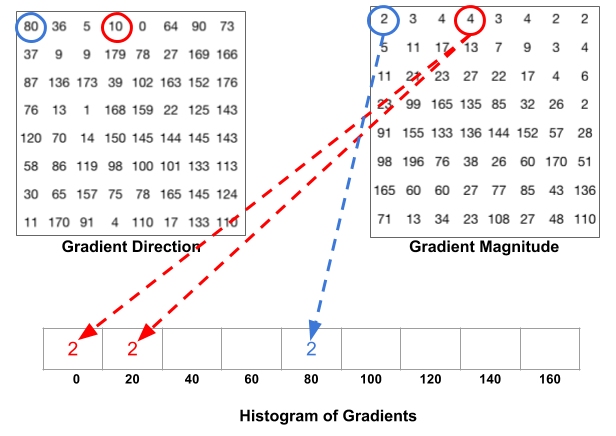
\includegraphics[width=10cm]{zdjęcia/gradients-histogram.png}
	\caption{Schemat tworzenia histogramu dla komórki o wymiarach $8x8$ \cite{hog2}} 
	\label{fig:gradientHistogram}
\end{figure}

Po wykonaniu procesu dla wszystkich pikseli można zobaczyć w jaki sposób rozkładają się wartości w zależności od kierunku gradientu charakteryzującego każdy z nich. Taka reprezentacja zapewnia odporność na szum, który istnieje między gradientami na samym początku. 

Gradienty obrazu są wrażliwe na oświetlenie. W przypadku zmiany jego natężenia, ich wielkość diametralnie się zmienia. Aby uodpornić deskryptor na jego wpływ stosuję się normalizację histogramu. 

Bloki przekształca się w wektory elementów, a następnie dla każdego stosuje się normalizację. Blok o wymiarach $16x16$ posiada 4 histogramy, gdzie każdy da się przedstawić jako wektor $9x1$ co w sumie daje wektor $36x1$. Normalizacja następuje dla pierwszego okna, po czym jest ono przesuwane o 8 pikseli gdzie znormalizowany wektor jest obliczany ponownie. Wszystko powtarza się do momentu przebycia wszystkich pozycji.

Każdy z omawianych bloków reprezentowany jest przez wektor $36x1$ co jest równoznaczne z 36 wyodrębnionymi cechami. Istnieje 105 pozycji takich bloków (7 poziomych, 15 pionowych). Sumarycznie, dla naszego zdjęcia, otrzymujemy aż 3780 cech.

Powyżej zostało opisane działanie deskryptora HOG na pojedynczym obrazie. Jest on podstawą rozpatrywanego algorytmu, którego celem jest stworzenie programu wykrywającego twarze. Aby osiągnąć takową użyteczność, należy połączyć działanie deskryptora z klasyfikatorem SVM.

Klasyfikator SVM pozwala na analizę danych, rozpoznanie wzorców i ich klasyfikację. Do jego wytrenowania używa się próbek pozytywnych i negatywnych, tak jak w przypadku przygotowywania klasyfikatora kaskadowego.

Z każdego zdjęcia, za pomocą deskryptora, należy wyciągnąć cechy HOG. Na ich podstawie trenuje się klasyfikator SVM. Uczy on się różnych możliwych cech twarzy, które potem próbuje zlokalizować na nowym zdjęciu. Po fazie uczenia, klasyfikator pozwala określić do jakiej klasy należą przetwarzane dane. W naszym przypadku rozróżni on fragment zawierający twarz i ten na którym się ona nie znajduje. 

Analizowana w tej sekcji metoda stała się konkurecją dla algorytmu opisywanego we wcześniejszym podrozdziale. Dokładność jego działania jest dużo lepsza niż algorytmu opartego na klasyfikatorze kaskadowym. Minusem jest wykrywanie twarzy tylko w przypadku widoku z przodu, program nie działa poprawnie w momencie jej rotacji i zmian kąta. Podobnie jak algorytm przedstawiony w poprzednim rozdziale, to podejście wciąż cieszy się wielką popularnością. Opracowane rozwiązanie zdaje się być proste i efektywne.

% %---------------------------------------------------------------------------

\section{Identyfikacja punktów charakterystycznych}
\label{sec:landmarks}
Opisana wcześniej technika wykrywania twarzy jest początkowym etapem działania rozwiązania, które zostanie przedstawione w niniejszej sekcji. Mowa tutaj o algorytmie detekcji punktów charakterystycznych twarzy (ang. facial landmarks), poprzez których pojęcie rozumie się elementy, pomagające zidentyfikować jej najistotniejsze cechy. Zazwyczaj są to punkty utożsamiane z linią szczęki, ust, nosa, oczu i brwi \cite{landmarks2}.

Schemat wykrywania owych elementów działa dwuetapowo. Pierwszym krokiem jest lokalizacja twarzy. Metoda, która zostanie do tego wykorzystana nie jest istotna. Ważne jest uzyskanie ograniczonego obszaru, aby następnie można było rozpocząć wykrywanie kluczowych struktur. 

Tak jak w innych przypadkach, istnieje wiele różnych propozycji rozwiązania tego problemu. Algorytm, który aktualnie cieszy się dużą popularnością został zaproponowany w 2014 roku, a jego działanie opiera się na wykorzystaniu drzew regresji. Jego autorami są Vahid Kazemi oraz Josephine Sullivan \cite{landmarks}. 

\begin{figure}[h]
	\centering
	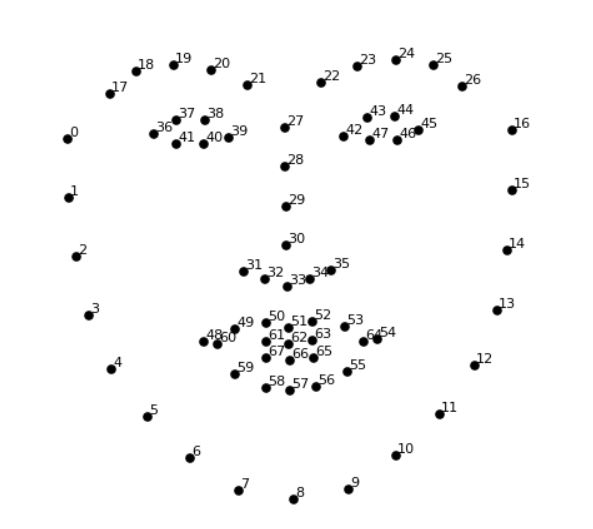
\includegraphics[width=8cm]{zdjęcia/landmarks_points.JPG}
	\caption{Wizualizacja 68 punktów charakterystycznych twarzy \cite{landmarksPoints}}
	\label{fig:landmarks}
\end{figure}

Działanie tej techniki można opisać w następujący sposób:
\begin{enumerate}
    \item Jako zbiór testowy wybiera się taki zestaw danych, który składa się z obrazów z oznaczonymi ręcznie punktami charakterystycznymi twarzy.
    \item Następnie model zostaje szkolony za pomocą drzew regresji na podstawie samej intensywności pikseli i próby dopasowania punktów w odpowiednie miejsca.
    \item  Korzysta się z obliczania prawdopodobieństwa odległości między parami pikseli.
    \item Celem treningu jest optymalizacja funkcji błędu i dokonanie selekcji odpowiednich cech w oparciu o dane zawarte w zbiorach.
\end{enumerate}

Rezultatem powyższych działań jest model zdolny do zlokalizowania charakterystycznych obszarów twarzy. W artykule, w którym pierwszy raz zaproponowano to rozwiązanie, testowano algorytm na zbiorze danych umożliwiającym wykrycie aż 192 istotnych punktów. Popularne biblioteki, w tym dlib, często udostępniają wariant wytrenowany na innym zbiorze danych. Zazwyczaj są to obrazy, na których oznaczono 68 kluczowych pozycji punktów (Rys. \ref{fig:landmarks}).

Zaletą przedstawionego algorytmu jest niezwykle szybki czas działania oraz dobra dokładność wykrywania elementów, nawet w przypadku twarzy ukazanych z profilu. Plusem jest także możliwość użycia dowolonych danych treningowych, czego efektem jest wyszkolenie własnego detektora punktów nie tylko twarzy, ale też innych niestandardowych elementów.

Technika, która została omówiona w tym rozdziale znajduje swoje zastosowania w wielu dziedzinach życia. Często jest ona uzupełnieniem wykrywania twarzy, w celu upewnienia się co do tożsamości danych osób. Jest to przydatny system w analizowaniu emocji ludzi, pozwala osobom z autyzmem bądź innymi chorobami lepiej zrozumieć otaczający ich świat. W przypadku oprogramowania czytającego z ruchu warg również analizuje się zmiany lokalizacji ważnych punktów charakterystycznych \cite{fDetection2}.

% %---------------------------------------------------------------------------

\section{Triangulacja Delaunaya}
Poprzez pojęcie triangulacji, w kontekście matematycznym, można rozumieć podział figury geometrycznej na trójkąty, bądź też czworościany (określane jako sympleksy) w taki sposób, aby część wspólna dwóch sąsiadujących trójkątów (czworościanów) była ich wspólną ścianą, wierzchołkiem, bokiem, trójkątem lub zbiorem pustym \cite{triangulation}.

Istnieje wiele różnych rodzajów triangulacji. W przypadku rozważanego w tej pracy algorytmu wykorzystano triangulacje zbioru punktów w przestrzeni 2D, do której należy między innymi triangulacja Delaunaya (lub Delone), której nazwa pochodzi od nazwiska autora tejże koncepcji Borysa Delaunaya. 

Triangulacja Delone \cite{tDelone} rozumiana jest jako triangulacja $T$ przestrzeni $R^{n+1}$, którą definiuję się w poniższy sposób. Jako $T$ określa się podział przestrzeni $R^{n+1}$ na $(n+1)$ trójkątów, z punktami jako wierzchołki, spełniających okreśone warunki:

\begin{enumerate}
    \item Każde dwa trójkąty należące do zbioru $T$ posiadają wspólną ściane albo nie są ze sobą połączone w żaden sposób.
    \item Każdy z ograniczonych zbiorów w przestrzeni $R^{n+1}$ ma część wspólną z ograniczoną liczbą trójkątów ze zbioru $T$.
    \item Opisując kulę na dowolonym trójkącie ze zbioru $T$ nie natkniemy się na sytuację, gdy wnętrze kuli będzie zawierało wierzchołki z pozostałych sympleksów zawartych w zbiorze $T$.
\end{enumerate}

\begin{figure}[h]
	\centering
	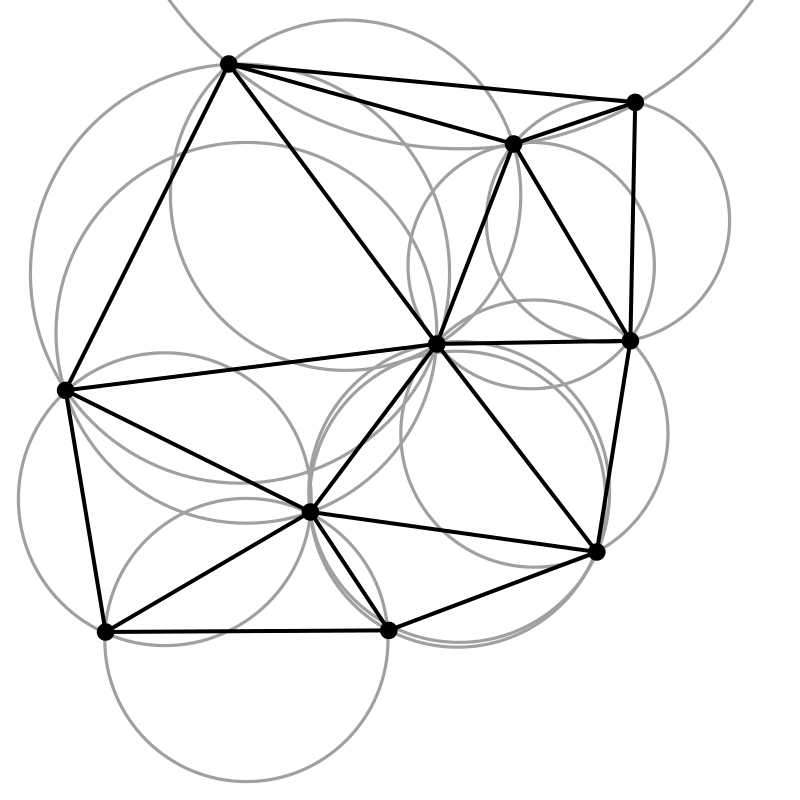
\includegraphics[width=6cm]{zdjęcia/triangulation.png}
	\caption{Przykładowa triangulacja Delone dla zbioru punktów \cite{tDelone}}
	\label{fig:delone}
\end{figure}

Przedstawioną powyżej koncepcję można uogólnić do przestrzeni o większych wymiarach. Wspominając o triangulacji Delone warto także wspomnieć o diagramach Voronoia, które są ściśle powiązane z owym pojęciem. Diagram, dla zestawu punktów, dzieli przestrzeń w taki sposób, że linie podziału znajdują się w równej odległości od punktów sąsiadujących.

Ważną własnością trangulacji Delone jest fakt, iż wraz z diagramem Voronoia tworzy graf dualny. Te definicje są powiązane, więc znając trangulację Delone dla zbioru punktów możemy w łatwy sposób obliczyć diagram Voronoia. Dwa trójkąty mające wspólną krawędź w triangulacji umożliwiają odnalezienie krawędzi w diagramie Voronoia. 

Centra okręgów wyznaczonych przez owe trójkąty po połączeniu tworzą daną krawędź. Rys. \ref{fig:voronoi}  przedstawia krawędzie triangulacji (czarne linie) oraz utworzone na podstawie triangulacji komórki Voronoia (czerwone linie).

\begin{figure}[h]
	\centering
	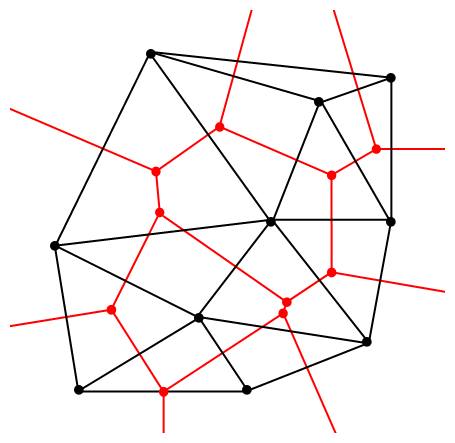
\includegraphics[width=6cm]{zdjęcia/voronoi.png}
	\caption{Graf przedstawiający komórki Vornoia oraz krawędzie triangulacji \cite{tDelone}} 
	\label{fig:voronoi}
\end{figure}

Istotną własnością tej techniki jest fakt, że trójkąty powstałe w wyniku triangulacji nie mają kątów o dużych miarach, co zapewnia przejrzystość wygenerowanych figur. W przypadku zastosowania triangulacji na zbiorze punktów można uniknąć chaosu i nierównomierności.

Triangulacja ma swoje zastosowania w wielu dziedzinach. Wykorzystuje się ją w informatyce, grafice komputerowej czy też geodezji. Technika umożliwia tworzenie skomplikowanych figur, wypełnianie obszarów, wyznaczanie linii przecięcia.

Istnieje wiele różnych algorytmów przeznaczonych do znajdowania trangulacji Delone dla zbioru punktów. Przedstawienie ich w niniejszej pracy dyplomowej nie jest jednak kluczowe. Większość języków programowania dostarcza odpowiednie biblioteki, które posiadają funkcje implementujące takowe algorytmy. 


